\newprob{1717151252}
{
    一個水波槽中有深水區和淺水區。一個波源以 20 Hz 產生一列向右傳播的直線波,如圖中所示。\\In a water tank, there are deep water and shallow water regions. A wave source generates a straight wave propagating to the right at a frequency of 20 Hz, as shown in the diagram.
    \par{\par\centering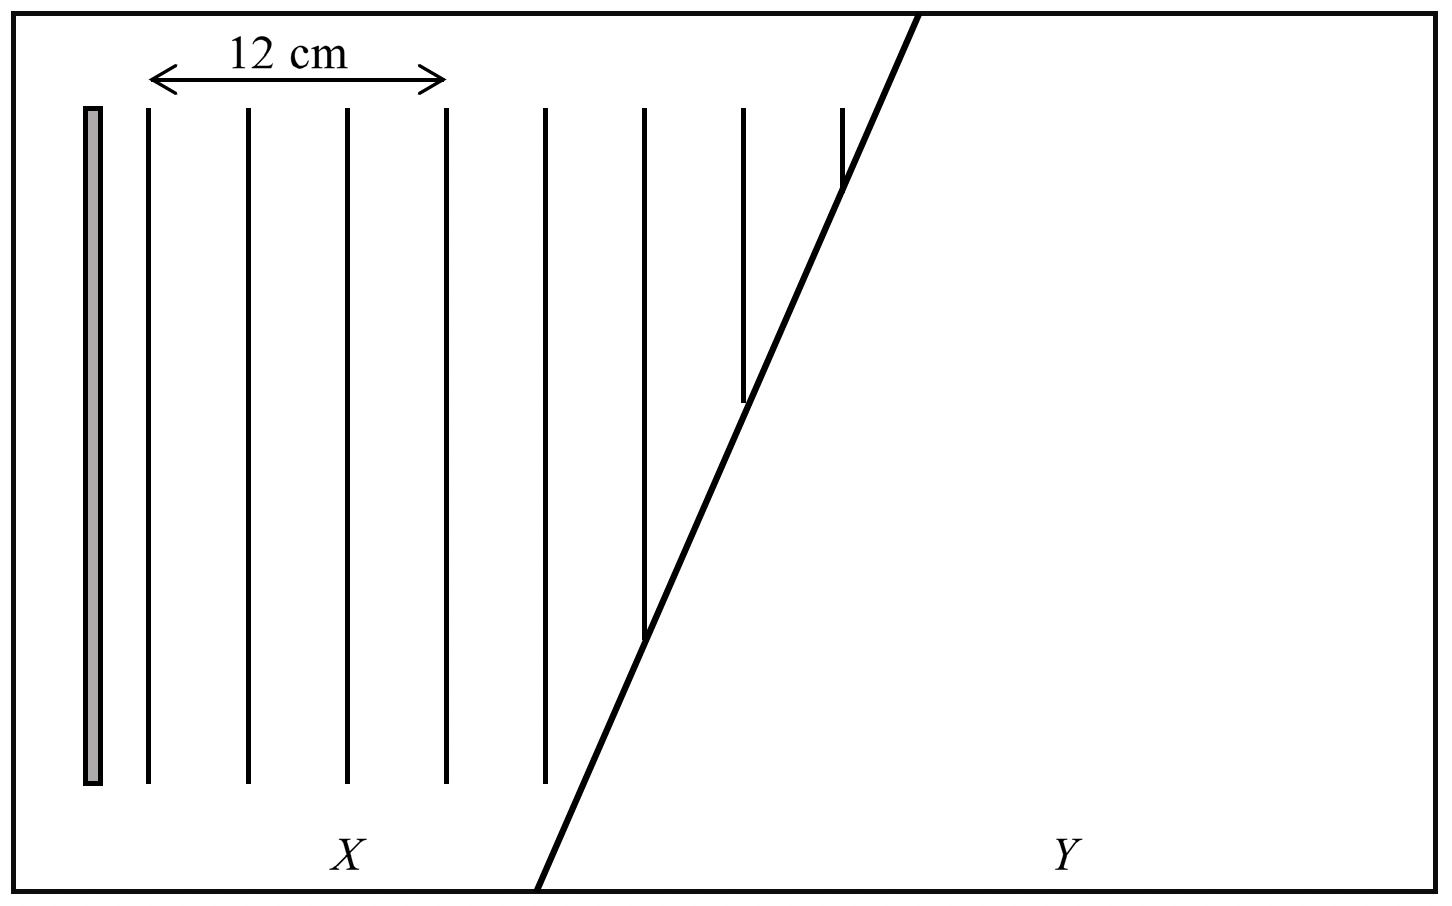
\includegraphics[width=.65\textwidth]{./img/ch2_weekend_lq_2024-05-31-19-20-09.png}\par}
    \begin{parts}
        \part 計算水波在區域X中的波速。\\Calculate the speed of water wave in region X.
        \zh{2}
        \part 水波在區域Y中的波長是 2 cm。\\Wavelength of water wave in region Y is 2 cm.
        \begin{subparts}
            \subpart 區域X和區域Y哪個區域較深水?寫出你的答案。\\Which region (X or Y) is deeper? Write down your answer.
            \zh{1}
            \subpart 在圖中畫出水波在區域Y的波陣面。\\Draw the wavefront of water wave in region Y.
            \zh{2}
            \subpart 寫出水波在區域Y的頻率。\\Write down the frequency of water wave in region Y.
            \zh{1}

        \end{subparts}
        \part 若在水波槽中加水,描述波陣面在區域X或有的改變,並扼要解釋你 的答案。\\When water is added to the tank, describe the change of wavefront in region X, explain your answer briefly.
        \zh{2}
        \part 若水波在水波槽的邊緣發生反射,或會影響觀察。寫出一項水波槽的改良 設計以減輕水波反射造成的影響。\\The observation can be affected when some water wave reflected at the edge of the water tank. Write down one modification design to the water tank to reduce this reflection.
        \zh{1}
    \end{parts}
    \dlines{1}\clearpage
}{
    \begin{enumerate}
        \item $\lambda=12/3=\qty{4}{cm}$ \giveM
              \\$v=4\times 20=\qty{80}{cm.s^{-1}}$\giveA
        \item \begin{enumerate}
                  \item X\giveA
                  \item \topalign{\par\centering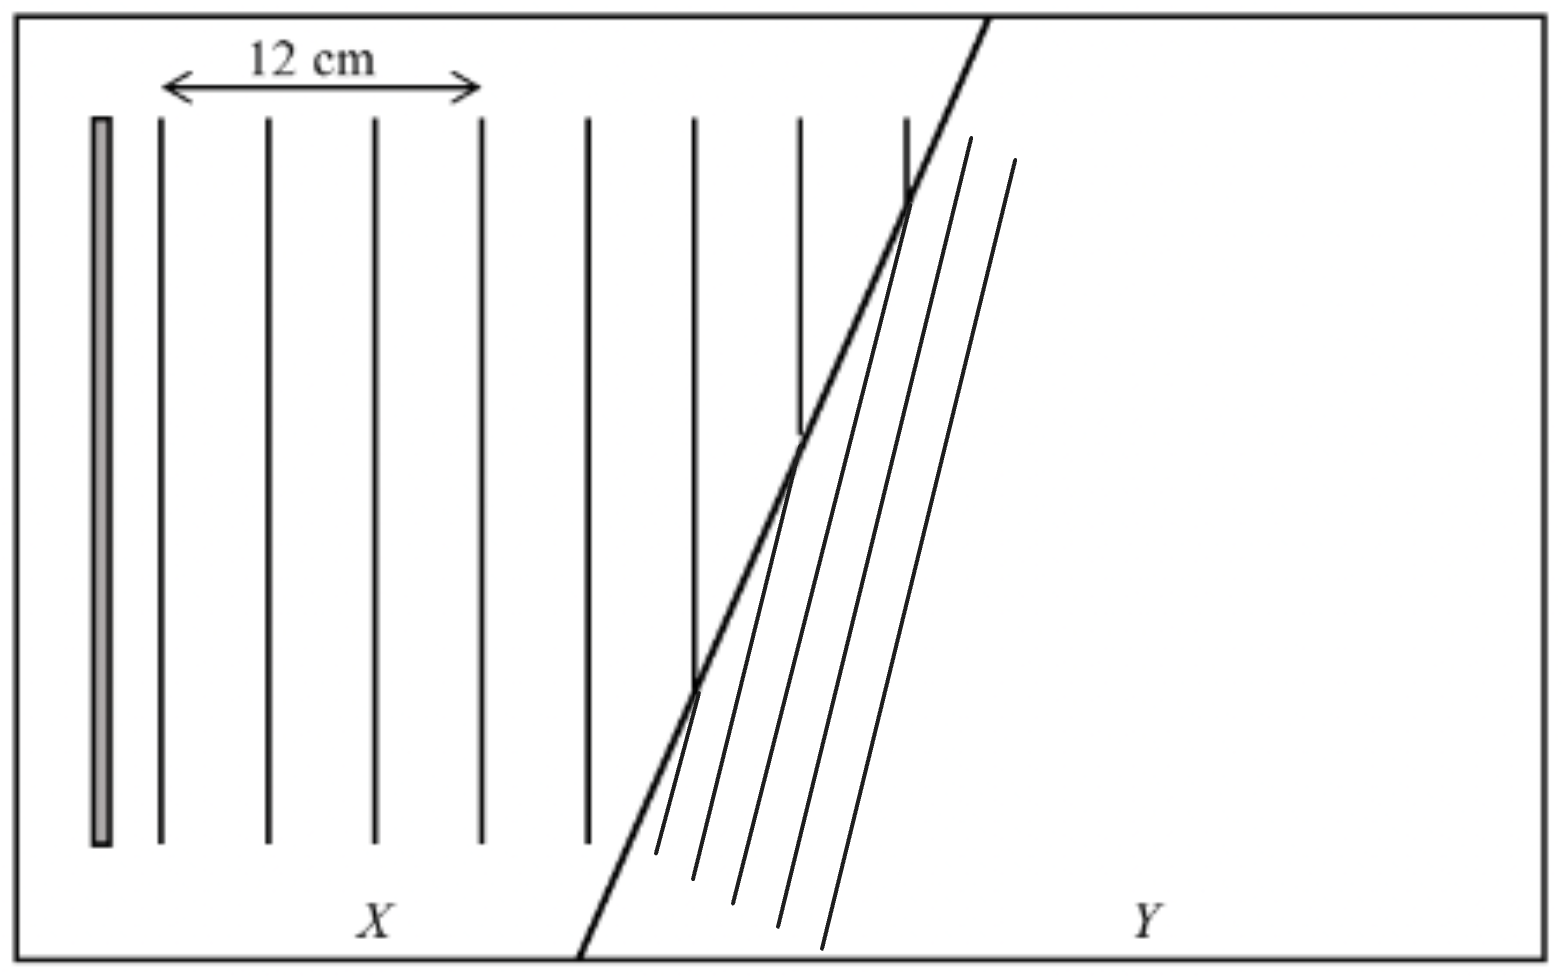
\includegraphics[width=.6\textwidth]{./img/ch2_weekend_lq_2024-06-01-00-28-00.png}\par}
                        \giveMA
                  \item \qty{20}{Hz}\giveA
              \end{enumerate}
        \item 波速增加,\\speed of wave increases,\giveM
              \\根據$v=f\,\lambda$,波長增加,波陣面間距增加。\\ by $v=f\,\lambda$, wavelength increases, separation between neighbouring wavefront increases.\giveA
        \item 在水波槽內壁加上海綿。
              \\ Add sponges to inner walls of water tank.\giveA
    \end{enumerate}
}